\documentclass{ECOS_2021}
%\usepackage{timesnew}
\usepackage{times}
\usepackage{graphicx}
\usepackage{amsmath}
\usepackage{amsfonts}
\usepackage{amssymb}
\usepackage{mathtools}
\usepackage{enumitem}
\usepackage{cite}
\usepackage{gensymb}
\makeatletter
\let\NAT@parse\undefined
\makeatother
\usepackage{hyperref}
\usepackage{float}
\usepackage{babel}
\usepackage[format=plain,
            labelfont=it,
            textfont=it,
		   font=small]{caption}

\renewcommand{\rmdefault}{phv} % Arial
%\renewcommand{\sfdefault}{phv} % Arial

\title{\sffamily A thermodynamic and technical feasibility study of subsurface storage of energy in the North Sea abandoned reservoirs}
\rmfamily
\author{Ali A. Eftekhari$^{a}$}

%\heading{First A. Author, Second B. Author and Third C. Author}

\address{$^{a}$ Technical University of Denmark,
Lyngby,
Denmark,
aliak@dtu.dk}

\abstract{\normalsize The oil and gas extraction from the Danish sector of the North Sea
has been declining, which will lead to the cessation of production
and abandonment (i.e., plugging of the wells and removal of the facilities).
Simultaneously, the existing and in development offshore windmills
in the North Sea will ensure the availability of abundant and cheap
electricity in the region yet fail to address the intermittent nature
of the wind resources. This paper hypothesizes that the surplus electricity
in the windy days and off-peak time can be converted to physical (compressed
hot fluids) or chemical (synthetic fuels, e.g., hydrogen, ammonia,
methanol, or methane) forms and stored in the vast space of the abandoned
oil and gas reservoirs under the North Sea. The stored energy can
be extracted and consumed as carbon-neutral fuels or be converted
back to electricity when there is a shortage of wind. This work studies
the technical and thermodynamic feasibility of offshore conversion
of electricity to physical and chemical energy sources and their storage/extraction
in/from the North Sea oil and gas reservoirs. The technical feasibility
study deals with the sufficiency of the existing infrastructures including
platforms, pipelines, and surface facilities to accommodate the process
equipment for the conversion of electricity to physical and chemical
storable forms. Several processes including nitrogen and carbon dioxide
separation from the atmosphere, electrolysis of seawater, and reduction
of CO$_{2}$ and N$_{2}$ to synthetic fuels are simulated in a commercial
process simulator. The simulation results are used for the sizing
of process equipment and the calculation of required platform area.
The thermodynamic analysis quantifies the exergy loss during the offshore
conversion, transportation, and storage/extraction of physical and chemical energy in the reservoirs based on the results of an in-house
opensource dynamic model that simulates the multi-component non-isothermal
flow of fluids in the subsurface. The results will finally estimate
the amount of wind electricity, offshore installations, and subsurface
space that is required to make Denmark self-sufficient and independent
of fossil fuels.}

\keywords{\normalsize Exergy analysis, Electricity to fuel, energy storage, Energy transition}

\begin{document}

% \thispagestyle{empty}

\sffamily \section{Introduction} \label{chap:Problem-definition} 
 \normalsize
Wind electricity is an intermittent and volatile source of energy
\cite{gibescuEstimationVariabilityPredictability2009,ummelsImpactsWindPower2007}.
When there is no or little wind, there is not enough electricity to
match the demand; when there is too much wind, if the electricity
is not consumed immediately, it will be wasted. The Ciara storm in
February 2020, which was only partially felt in Denmark, increased
the Danish wind electricity production to 1000 Mega Watts (MW) above
consumption, i.e. 20\% higher that is equivalent to the average demand
of one million European citizens. There were reports of significant
curtailments up to several thousand MW from other countries in the
North Sea region. Curtailment \cite{lewWindSolarCurtailment2013},
which means accepting less renewable electricity than what windfarms
can deliver is another word for wasted resources. It will soon become
more severe when the North Sea is hit by a technological storm in
the form of several large wind farms that are currently evaluated,
planned, and licensed \cite{GlobalOffshoreRenewable}. More importantly,
since the electricity distribution is planned based on the unavailability
of wind resources, the biomass (that is regularly switched to coal)
power plants must always be running to compensate for the shortage
of wind, thus emitting a large amount of carbon dioxide and other
pollutants \cite{meibomEnergyComesTogether2013}. The solution is
to store electricity when production is higher than demand and consume
it when demand is higher than production \cite{pedersenEnergyStorageTechnologies2019}. 

The oil and gas extraction from the Danish sector of the North Sea
has been declining, which will lead to the cessation of production
and abandonment (i.e., plugging of the wells and removal of the facilities).
Simultaneously, the existing and in development offshore windmills
in the North Sea will ensure the availability of abundant and cheap
electricity in the region yet fail to address the intermittent nature
of the wind resources. This paper hypothesizes that the surplus electricity
in the windy days and off-peak time can be converted to chemical energy
(synthetic fuels, i.e. hydrogen, ammonia, methanol, or methane) forms
and stored in the vast space of the abandoned oil and gas reservoirs
under the North Sea. The stored energy can be extracted and consumed
as carbon-neutral fuels for transportation or be converted back to
electricity when there is a shortage of wind. This paper studies the
technical and thermodynamic feasibility of offshore conversion of
electricity to chemical energy sources. The technical feasibility
study deals with the sufficiency of the existing infrastructures including
platforms, pipelines, and surface facilities to accommodate the process
equipment for the conversion of electricity to chemical storable forms.
Several processes including nitrogen and carbon dioxide separation
from the atmosphere, electrolysis of seawater, and reduction of CO$_{2}$
and N$_{2}$ to synthetic fuels are simulated in Aspen Plus process
simulator. The simulation results are used for the sizing of process
equipment and the calculation of required platform area. The thermodynamic
analysis quantifies the exergy loss during the conversion of electricity
to fuel and back, and storage/extraction of chemical energy in the
reservoirs based on the results of an in-house opensource dynamic
model that simulates the multicomponent non-isothermal flow of fluids
in the subsurface \cite{eftekhariFVToolFiniteVolume2015b}.

There are three major questions that will be answered in this work.
First, how much energy storage is needed in Denmark? Secondly, to
what extent can the subsurface storage be helpful in addressing the
intermittency of the renewable electricity? Thirdly, what are the
promising technologies from a technical point of view? This paper
will provide simple, reproducible, and realistic procedures and quantitative
answers to these questions.

\sffamily \section{Future energy need of Denmark}
\normalsize

The current plan is to quadruple the current
electricity production capacity of the windmills in the North Sea. Since the
capacity is not equal to the actual produced electricity (due to,
e.g. technical problems, curtailment, weather conditions, etc.) we
will estimate the intermittent electricity production of the windmills
by quadrupling the current electricity production in Denmark that
is available from Energinet.dk website and also available as a public
repository \cite{eftekhariSimulkadeStorageFirst2021}, including several
Matlab functions for analysis and visualizations. We can also assume that the 
domestic transport and heating will be fully electrified by 2050, which will add 50\% 
to the current electricity demand \cite{eftekhariQuantifyingRoleLiquid2020}.

Fig. \ref{fig:Electricity-surplus-smooth} shows the electricity supply
and demand from May 2021 to January 2021 (left) and for the same period
in 2050 (right). We can use Eq. (\ref{eq:average-energy-demand})
to integrate the data and obtain the average energy supply and demand
over different periods of time, i.e. from 24 hours to nine month,
as shown in Fig. \ref{eq:average-energy-demand}:
\begin{equation}
\bar{E}=\frac{1}{t_{2}-t_{1}}\int_{t_{1}}^{t_{2}}E\left(t\right)dt,\label{eq:average-energy-demand}
\end{equation}
where $E(t)$ {[}MW{]} is the electricity supply or demand in the
future and $t_{1}$ {[}s{]} and $t_{2}$ {[}s{]} represent a certain
time period. The future energy supply and demand are estimated by
using the correction factor extracted from \cite{eftekhariQuantifyingRoleLiquid2020},
e.g.
\begin{equation}
E_{future}=\lambda_{i}E_{current},\quad i=s,\,d\label{eq:demand-adjust}
\end{equation}
where $\lambda_{d}=1.5$ denotes a 50\% in electricity demand \cite{eftekhariQuantifyingRoleLiquid2020}
and $\lambda_{s}=4.0$ denotes a 400\% increase of windmill capacity
in Denmark \cite{danishenergyagencyEnergyIslands2021,dandreaSynergiesOffshoreEnergy2021}.
Note that this increase will be on the offshore sector only; however,
here we assume that the overall wind energy capacity will increase
by a factor of four. The other assumption in Eq. (\ref{eq:demand-adjust})
is that the weather (more specifically, wind) in 2050 will be similar
to the weather condition in 2020. The visualized energy supply and
demand in Fig. \ref{fig:Electricity-surplus-smooth} shows that periodically,
the wind electricity supply is higher or lower than the electricity
demand, creating periods with electricity surplus and shortage, respectively.
The alternation between surplus and shortage can occur within a few
hours to few weeks. This is better visualized in Fig. \ref{fig:Average-electricity-supply}
that shows the average surplus and shortage for periods of 24 hours
to 8 months. It can be observed that after around six months, the
average surplus and shortage reach a constant value. This plot unveils
three critical pieces of information about the wind electricity supply
and demand in 2050: first, the average shortage of electricity is
1.6 GW, which is a large amount of power and gives an indication of
the amount of energy that needs to be stored (although sometimes the
actual power shortage is temporarily higher as shown later). The good
news is that the average electricity surplus is 2.25 GW, which is
620 MW higher than the average electricity shortage. These two numbers,
however, serve as a constraint for the efficiency of the energy storage
technology, i.e.
\[
\eta_{storage}>\frac{\text{Average shortage}}{\text{Average surplus}}=0.72.
\]
This means that the efficiency of the storage technology must be higher
than 72\%.

\begin{figure}[H]
\centering
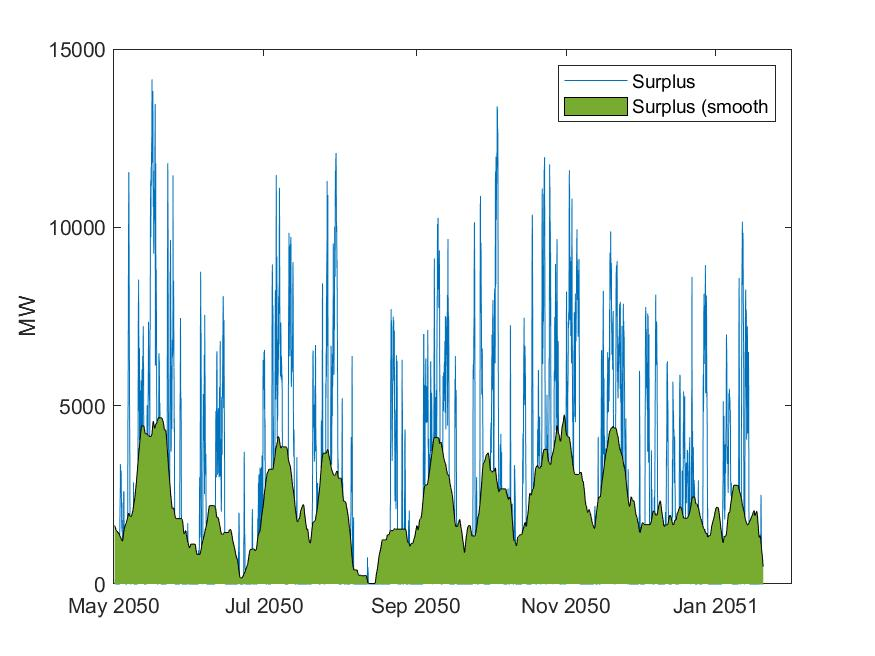
\includegraphics[width=8cm]{smoothed_surplus}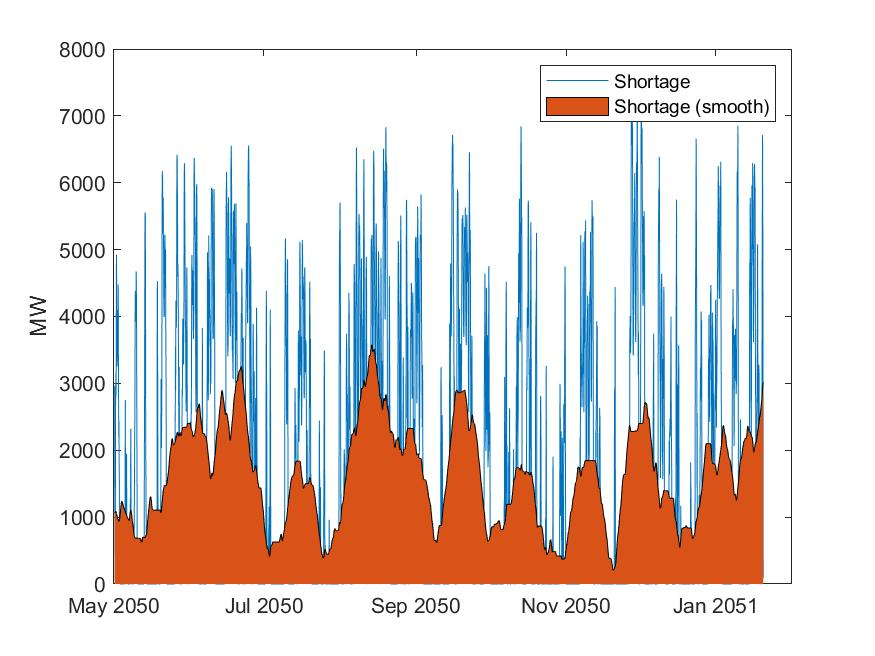
\includegraphics[width=8cm]{smoothed_deficit}

\caption{\label{fig:Electricity-surplus-smooth}Electricity surplus (left)
and shortage (right) adjusted for 2050; the smoothed curve is shown
by area plot.}
\end{figure}

\begin{figure}[H]
\centering
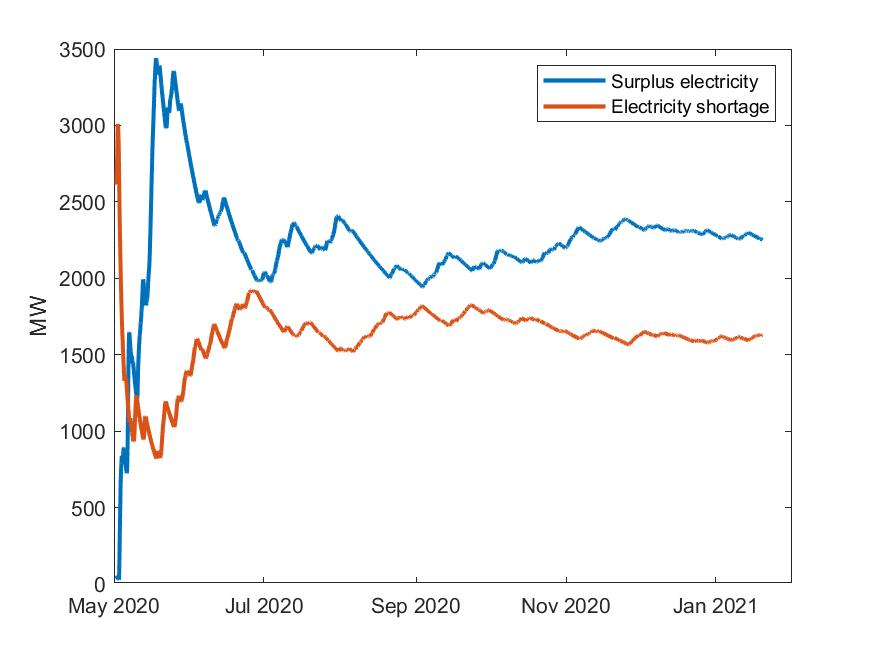
\includegraphics[width=8cm]{supply_demand_six_month_dk}

\caption{\label{fig:Average-electricity-supply}Average electricity supply
and demand for Denmark adjusted for May 2050 to January 2051; see
Eq. (\ref{eq:average-energy-demand})}
\end{figure}

Although the previous analysis provides the average storage value,
the real time electricity surplus that needs to be stored varies with
time. The same occurs with the electricity shortage, i.e. the occasional
electricity shortage can be much higher than its long-term average
value. Both of these values are shown in Fig. \ref{fig:Electricity-surplus-smooth}.
Any feasible storage process must be able to store a maximum power
surplus of 5.0 to 10.0 GW (see the peaks of the curves in Fig. \ref{fig:Electricity-surplus-smooth}-left)
and recuperate the stored power with a maximum rate of 3.0 to 6.0
GW (see the peaks of the curves in Fig. \ref{fig:Electricity-surplus-smooth}-right).
These values are critical in the design of the storage and recuperation
processes. The sizing of the required equipment and sub-processes
will be discussed in the next sections. 

We end this section by estimating the subsurface volume that is required
to store enough energy to cover for a eight month energy shortage.
Table \ref{tab:Exergy-value-efficiency} shows the exergy per unit
mole of different energy storage media that are studied in this paper.
Exergy, $ex_{i}$ {[}kJ/mol{]} is the amount of energy in a system
that can be converted to mechanical work, i.e. movement. The maximum
efficiency of producing each medium, $\eta_{i}$, is also reported
in Table \ref{tab:Exergy-value-efficiency}. For these calculations,
we need to have the density of the stored fluids at reservoir conditions,
$T_{res}$ {[}K{]} and $p_{res}$ {[}bar{]}. We used the typical reservoir
conditions of the chalk fields in the Danish sector of the North Sea,
i.e. 70$^{o}$C and 200 bar. The volume of the reservoir is calculated
by
\[
V_{res,i}=\frac{\bar{E}_{shortage}t_{storage}MW_{i}}{ex_{i}\rho_{i}\varphi},
\]
where $\bar{E}_{shortage}$ {[}kW{]} is the average electricity shortage,
$t_{shortage}$ {[}s{]} is the period over which the electricity shortage
is estimated (here 8 months), $MW_{i}$ {[}kg/mol{]} is the molecular
weight of the stored fluid, $\rho_{i}$ {[}kg/m$^{3}${]} is the density
of the stored fluid at reservoir condition, and $\varphi$ {[}-{]}
is the porosity of the reservoir. Assuming a reservoir thickness of
100 m, the diameter of a chalk reservoir that can store the equivalent
of eight-month electricity shortage in 2050 is calculated. The diameter is calculated assuming
an efficiency factor of one for all the energy conversions. A 2 to
3 times larger reservoir volume is required if all the efficiency
factors are included in the computations. All in all, the required
volume for the energy storage is only a small fraction of the available
reservoir volumes in the North Sea. Therefore, the reservoir volume
is not a bottleneck in the subsurface energy storage. A reservoir
with a thickness of 100 m and a radius between 100 m to 3000 m (considering
the efficiency factors) can hold enough energy to compensate for 8
months of electricity shortage in Denmark in 2050. 

\begin{table}[h]
\normalsize
\caption{\label{tab:Exergy-value-efficiency}Exergy value and the efficiency
of producing different energy storage media and the thermodynamic
properties at reservoir condition (70$^{o}$C, 200 bar); the efficiency
factors are only considered for the electricity to fuel conversion.}

\begin{center}
\begin{tabular}{ccccc}
\hline 
Component & $\rho$ {[}kg/m$^{3}${]} & $ex$ {[}kJ/mol{]} & $V_{res}$ {[}10$^{6}$ m$^{3}${]} & $\eta$ {[}-{]}\tabularnewline
\hline 
NH$_{3}$ & 667.7 & 340 & 2.50 & 0.45\tabularnewline
CH$_{4}$ & 386.6 & 831 & 1.66 & 0.36\tabularnewline
H$_{2}$ & 67.7 & 236 & 4.21 & 0.7\tabularnewline
CH$_{3}$OH & 871.2 & 720 & 1.70 & 0.4\tabularnewline
Air & 733.5 & 22.0 & 59.89 & 1.0\tabularnewline
\hline 
\end{tabular}
\end{center}
\end{table}

\sffamily \section{Synthetic fuel storage}
\normalsize

The conversion of electricity to carbon-neutral fuels, known as power2x,
p2x, e-refinery, and several other names, is a topic that is extensively
studied, e.g. \cite{freiMethanolHydrogenCarrier2020b,ghaibPowertoMethaneStateoftheartReview2018,guerraMethaneProductionCombined2018,koponenReviewWaterElectrolysis2015,mendoza-hernandezExergyValorizationWater2019}.
To produce a carbon-neutral fuel, the raw material for the production
of the synthetic fuels must come from the dead state, i.e. atmosphere
and sea water. The dead state refers to the average composition of
the atmosphere, Earth's crust, and oceans that theoretically does
not have any potential to do work. Here, we consider the production
of hydrogen, ammonia, methane, and methanol. The raw material for
the production of these fuels are air and seawater and the only driving
force for the production processes is the surplus electricity from
the windfarms. From the atmosphere, nitrogen and carbon dioxide need
to be separated. From the seawater, hydrogen will be extracted via
an electrolysis process. These processes are discussed in the next
section.

\sffamily \subsection{Nitrogen}
\normalsize
Nitrogen can be extracted from the air through the cryogenic distillation
of air. In this process, shown in Fig. \ref{fig:Ammonia-synthesis-cryogenic},
air is filtered, compressed, and liquefied by passing through a series
of heat exchangers. The liquefied air then enters a high pressure
followed by a low pressure distillation column. The separation of
nitrogen from oxygen and other minor constituents of air is done based
on the difference of their boiling points. Nitrogen is separated from
the top side of the low pressure column. To liquefy air, a utility
stream of around -200$^{o}$C is required, that is often provided
through the sudden expansion of a compressed refrigerant. Therefore,
the entropy generation is high and the process is exergy intensive.
Different values are reported in the literature for the electricity
consumption per unit mole of separated nitrogen. These values depend
on the heat integration of the process. The largest value reported
in the literature is around 15 kJ/mol air distilled. In our simulation,
we obtained a value of 32 kJ/mol, which is perhaps due to the poor
heat integration in the simplified simulations; thus, we used the
value of 15 kJ/mol in our analysis.

\begin{figure}[H]
\centering
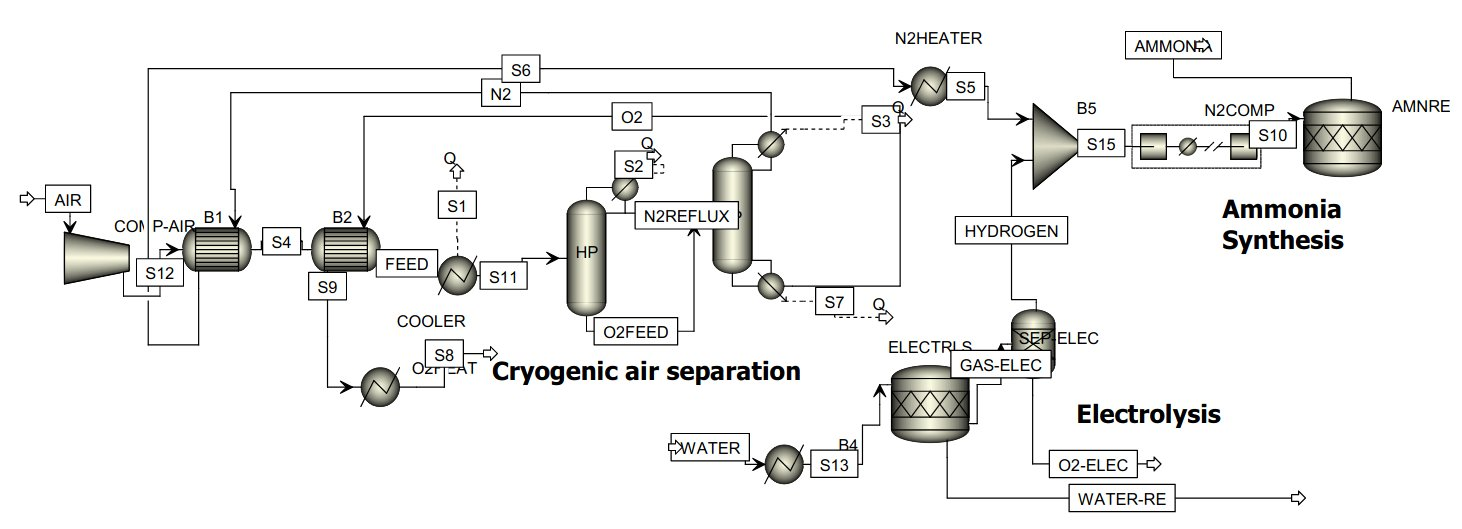
\includegraphics[width=14cm]{ammonia_cryogenic}

\caption{\label{fig:Ammonia-synthesis-cryogenic}Ammonia synthesis process
based on electrolysis and cryogenic air separation}
\end{figure}


\sffamily \subsection{Carbon dioxide}
\normalsize
Carbon dioxide is a stable molecule that exist in a small concentration
of around 40 ppm (40$\times$10$^{-6}$ mole fraction) in the atmosphere.
Theoretically, it can be separated from the atmosphere by spending
an energy amount that is equal to the chemical exergy of carbon dioxide
\cite{sankaranarayananEfficiencySustainabilityEnergy2010}, i.e.
\[
ex_{CO_{2}}=-RT_{00}\ln x_{CO_{2}},
\]
where $R$ {[}8.314 J/(mol.K){]} is the universal gas constant, $T_{00}$
{[}K{]} is the dead state temperature (15$^{o}$C or 288.15 K in the
North Sea region), and $x_{CO_{2}}$ is the mole fraction of CO$_{2}$
in the atmosphere. This gives a value of 18744 J/mol, or roughly 20000
J/mol. Based on the previous experiences in the gas industry for the
separation of low concentration acid gases such as CO$_{2}$, SO$_{2}$,
and H$_{2}$S, the efficiency of such a process is quite low and rarely
exceeds 5\% \cite{keithWhyCaptureCO22009a,mahmoudkhaniLowenergySodiumHydroxide2009}.
This means that the energy requirement for the separation of CO$_{2}$
from the atmosphere is around 400 kJ/mol or 9.0 MJ/kg CO$_{2}$. In
practice, this number is around 10 MJ/kg CO$_{2}$ which is both accurate
and memorable, although larger numbers are reported for the state
of the art technology \cite{internationalenergyagencyDirectAirCapture}.

Besides being energy-intensive, the separation of atmospheric CO$_{2}$
(also known as air capture) has a large footprint since a large mass
transfer area is needed between the air and adsorbents/absorbents;
the footprint of the equipment is between 0.5 to 2 km$^{2}$ for capturing
1 million ton of CO$_{2}$ per year \cite{DirectAirCapture2021,mcqueenCostAnalysisDirect2020}.
This means that the direct air capture equipment cannot fit on a platform.

There are other ways of providing -close to- CO$_{2}$-neutral carbon
sources, e.g. from biomass. The captured CO$_{2}$ from the industrial
point sources, e.g. steel and cement industries or fossil fuel power
plants, if the capturing and conversion to fuel is performed in a
close cycle can also be carbon-neutral. However, these two sources
are available onshore and it is therefore easier to utilize them as
close to the source as possible. The other source of carbon is the
remaining oil and gas in the reservoirs, which can be extracted by,
e.g. insitu combustion. However, this carbon source is not sustainable
and we will not consider it. 

\sffamily \subsection{Hydrogen}
\normalsize
Recent developments in the electrolysis technology has considerably
increased the efficiency of hydrogen production from water. If the
process is driven by the clean wind electricity, the produced hydrogen
is a zero-emission fuel. Currently, hydrogen is included in all the
energy scenarios for the countries in the North Sea region. For the
offshore hydrogen production and storage, the following aspects need
further investigations: fitting the water treatment, electrolysis,
and compression equipment on a platform; pipeline integrity (for storage
and gas transport); physico-bio-chemical interactions of hydrogen
with the formation fluids and the chalk reservoir; capacity of reservoirs
for storage of hydrogen and flow of hydrogen in the reservoir; energy
efficiency and economic value of the process. Here, the energy requirement
of the process, the size of the process equipment, and the flow of
hydrogen in the chalk reservoirs will be addressed. 

\sffamily \subsubsection{Green hydrogen production }
\normalsize
Hydrogen can be produced from the electrolysis of water in the following
reaction: 

\[
2H_{2}O\rightarrow2H_{2}+O_{2}.
\]

The minimum energy required for this reaction is given by the change
of Gibbs free energy \cite{rosenEnergyExergyAnalyses1995}. This reaction
requires 39 kWh of electricity per kg hydrogen, but with the state
of the art technology the value is closer to 48 kWh/kg \cite{gardnerHydrogenProductionRenewables2009,ozarslanLargescaleHydrogenEnergy2012}.

Hydrogen is purified by cooling it down to 308 K using cooling water.
It removes the moisture from the hydrogen stream. The condensed water
is recycled \cite{rosenEnergyExergyAnalyses1995}. Some extra moisture
remains in the hydrogen stream, which will be removed later in the
intercoolers between the compression stages \cite{rosenEnergyExergyAnalyses1995}.
Electricity must be provided as direct current (DC), which introduces
a loss of 2.5\% for AC-DC conversion \cite{rosenEnergyExergyAnalyses1995}.
Rosen assumes an exergy efficiency of around 70\% for the electrolysis
of water for a mature electrolysis technology in 1995 (not considering
other losses). He does not give more information on other steps of
the process, e.g. water treatment and purification. There are several
technologies to produce hydrogen from water using electricity among
which two are more mature and are available as commercial packages,
viz. alkaline electrolysis \cite{braunsAlkalineWaterElectrolysis2020}
and polymer electrolyte membrane cells (PEM) \cite{babicCriticalReviewIdentifying2017}.
If the electricity is supplied by renewable resources, the produced
hydrogen is called \textquotedblleft green hydrogen\textquotedblright{}
\cite{granovskiiExergeticLifeCycle2007}. An efficiency of 60\% to
70\% is expected for these electrolysis processes, in which most of
the energy loss is converted to heat. The energy loss during the compression
of hydrogen will be calculated separately in the following sections.

The storage of hydrogen in the subsurface is a relatively old topic
\cite{ozarslanLargescaleHydrogenEnergy2012,zivarUndergroundHydrogenStorage2020}.
Due to the high consumption of hydrogen, the petrochemical plants
have been using salt caverns to store large volumes of hydrogen in
the subsurface \cite{ozarslanLargescaleHydrogenEnergy2012}. Currently,
the subsurface storage of green hydrogen is being studied by several
investigators in different continents.

There are several green hydrogen
production projects being announced. Ørsted has announced that as
part of the project H2RES, supported by The Energy Technology Development
and Demonstration Programme (EUDP) under the Danish Energy Agency,
a hydrogen production unit with a 2 MW capacity will be built by the
end of 2021 \cite{OrstedTakesFinal} that will produce up to 1000
kg/day of green hydrogen. These capacities, although an step forward,
will not address the GW scale energy shortage that will certainly
occur due to the intermittent nature of renewable electricity, as
was discussed in section \ref{chap:Problem-definition}. 

The other issue that needs to be addressed here is the footprint of
the electrolysis equipment. We saw in section \ref{chap:Problem-definition}
that the synthetic fuel production units are expected to consume several
GW of surplus electricity. The main problem with these large amounts
of power is that the electrolysis units are currently designed and
built in MW scale. For example, one of the largest commercial PEM
electrolysis units offered by NEL hydrogen has a capacity of 25 MW
and requires 3$\times$12 m$^{2}$ area for installation. Therefore,
a 500 MW electrolysis plant that is made of 20 PEM cells is unlikely
to to fit on a platform with other equipment although it is not impossible.
A better option for the offshore hydrogen production is the installation
of these electrolysis cells onboard a ship designed for this purpose.
Otherwise, the onshore production of hydrogen seems to be the more
realistic option.

Last but not least is the conversion of the stored hydrogen to electricity.
Currently, there is no gas turbine that can work with pure hydrogen
as a fuel. Therefore, the produced hydrogen must be mixed with a hydrocarbon
fuel such as methane. This will cause some carbon dioxide emission
unless a carbon capture process is used, which will in turn reduce
the efficiency of the process. Fitting a GW scale turbine on a platform
is possible but similar to electrolysis cells highly unlikely for
GW capacities. As an example, Dan F host 6,800 tonnes of facilities
and provides a power of 55 MW to the facilities. The highest point
on the platform is 132 m above water. A typical 25 MW turbine that
is designed for offshore platforms and consumes a mixture of methane
and hydrogen weighs approximately 250 tonnes. Therefore, up to several
hundred MW of gas turbine capacity can fit on a platform. But reaching
to GW capacities can be a challenge.

\sffamily \subsection{Methane}
\normalsize
Methanation process for the catalytic conversion of CO$_{2}$ and
CO to methane was first suggested by Sendersen and Sabatier \cite{boltCriticalReviewSynthetic2020}.
The reaction occurs in multiple steps starting with capturing of CO$_{2}$
or from an industrial or natural source or producing a mixture of
CO$_{2}$ and CO by burning hydrocarbons (i.e. fossil fuels) or carbohydrates
(i.e. biomass). In the presence of water vapor and at high temperatures,
a considerable amount of CO and H$_{2}$ are also produced. H$_{2}$
can react with CO$_{2}$ and CO and convert them to methane. The reduction
of CO$_{2}$ to methane by hydrogen is known as Sabatier reaction
\cite{boltCriticalReviewSynthetic2020}: 

\begin{equation}
CO_{2}+4H_{2}\rightleftarrows CH_{4}+2H_{2}O\qquad\Delta H_{0}=-165\,\textrm{kJ/mol}.\label{eq:methane}
\end{equation}
If the reactants, i.e. hydrogen and CO$_{2}$ are obtained from the
dead state (i.e. seawater and atmosphere) using renewable electricity,
the produced methane is carbon-neutral and sustainable. The reaction
can be catalyzed by nickel or ruthenium and can be conducted in a
packed bed reactor. The reaction rate in different ranges of pressure
and temperature are reported in the literature. Although other reactions
can occur at the high temperature and pressure of the methanations
reactors, it is observed that the selectivity of the reaction towards
methane is high \cite{loderReactionKineticsCO22020}. A selectivity
of close to 100\% is observed for catalytic methanation of CO$_{2}$
over nickel catalyst at a temperature close to 300$^{o}$C. Although
theoretically the reaction reaches 100\% yield at room temperature,
in practice the reaction rate is too small and the methane yield is
zero. A temperature of at least 200$^{o}$C is needed to get the catalytic
reaction started. At temperatures above 500$^{o}$C, the reaction
goes backward, i.e. conversion of methane and water to hydrogen and
CO$_{2}$. This reaction is also known as methane reforming that is
currently the main reaction for the production of the so-called ``blue''
hydrogen, i.e. hydrogen that is produced from a hydrocarbon. A schematic
of the process for the production of green methane is shown in Fig.
\ref{fig:methane-process}. In this process, the required hydrogen
and carbon dioxide are produced by the electrolysis of water and separation
of atmospheric CO$_{2}$, respectively. The carbon source can also
be provided from other alternative sources such as biomass or from
the captured carbon dioxide from, e.g. cement or steel industries.
However, capturing CO$_{2}$ from the atmosphere has the benefit of
making the produced methane carbon-neutral or so-called ``green''.
The reactor pressure is 20-70 bar \cite{er-rbibModellingSimulationMethanation2013}
and the temperature is between 473 to 673 K. The overall efficiency
of the produced methane is calculated by
\begin{equation}
\eta_{methane}=ex_{CH_{4}}^{ch}\left(\frac{4ex_{H_{2}}^{ch}}{\eta_{electrolysis}}+\frac{ex_{CO_{2}}^{ch}}{\eta_{capture}}+\frac{ex_{compression}}{\eta_{comp}\eta_{driver}\eta_{transmission}}\right)^{-1},\label{eq:methane-efficiency}
\end{equation}
where $ex_{i}^{ch}$ {[}kJ/mol{]} denotes the chemical exergy of component
$i$, and $\eta_{j}$ {[}-{]} shows the exergetic efficiency \cite{eftekhariExergyAnalysisUnderground2012f}
of the process $j$; $ex_{compression}$ {[}kJ/mol methane{]} denotes
the exergy requirement for the compression of hydrogen and CO$_{2}$
to the pressure of the methanation reactor in a multistage compressor.
Since the reaction is exothermic, we assume that the heat of reaction
is sufficient to heat up the reactor to the required temperature of
673 K. By calculating the compression energy and replacing other efficiency
factors from the previous sections, we obtain $\eta_{methane}=36\%$.
This is much lower than the expected value of 72\%. Moreover, since
this process requires a large footprint for the direct atmospheric
capture of CO$_{2}$ and electrolysis of water, we do not consider
it as a feasible option that can address the intermittency of the
wind energy in Denmark. It is worth mentioning that this process can
easily fit on a platform and if both hydrogen and CO$_{2}$ are provided,
e.g. via pipelines, operating this process on a platform is viable.

\begin{figure}[H]
\centering
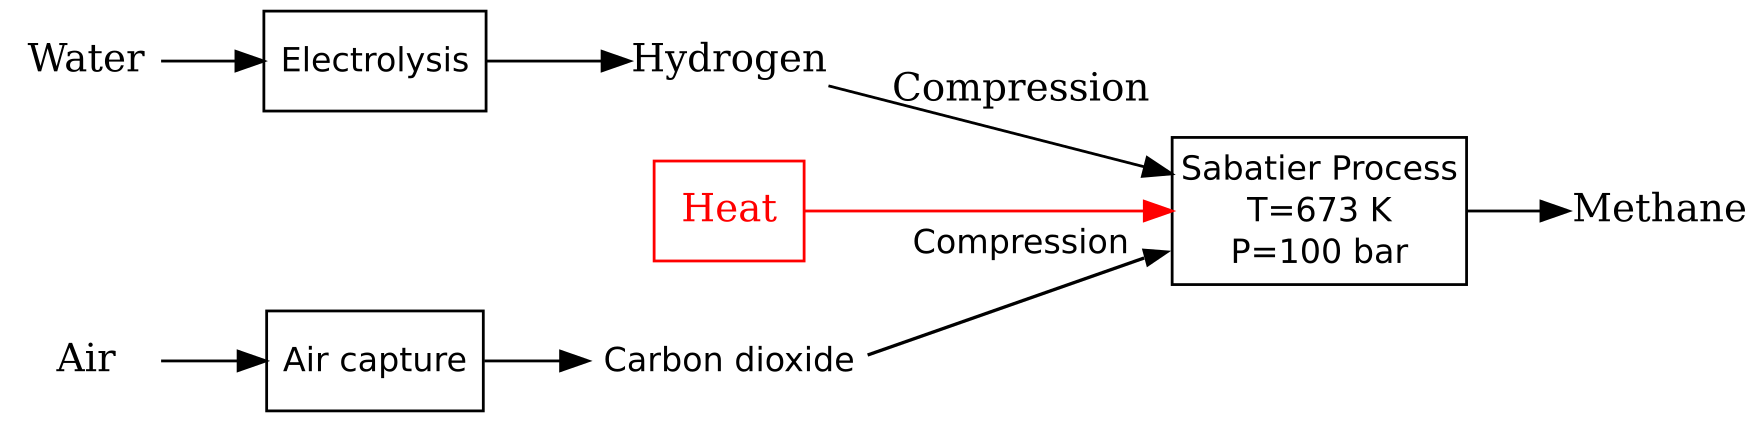
\includegraphics[width=12cm]{sabatier}

\caption{\label{fig:methane-process}A block flow diagram of Sabatier process
for the production of methane \cite{eftekhariQuantifyingRoleLiquid2020}}
\end{figure}


\sffamily \subsection{Ammonia}
\normalsize
The block flow diagram of ammonia production is shown in Fig. \ref{fig:Haber-process}.
Ammonia is produced by an exothermic catalytic reaction between nitrogen
and hydrogen:
\[
N_{2}+3H_{2}\rightarrow2NH_{3}.
\]
An ammonia reactor is operated at 200 bar and a temperature of 300
to 500$^{o}$C \cite{elnashaieSimulationOptimizationIndustrial1988,morudAnalysisInstabilityIndustrial1998}.
The raw material for the production of ammonia, i.e. nitrogen and
hydrogen, can be obtained from the air and seawater by the cryogenic
air separation and electrolysis units, respectively. The nitrogen
and hydrogen feed streams are compressed to 150 to 250 bar and react
in a packed bed reactor at 673 to 773 K. The reaction is exothermic
and therefore does not require external heating; it also produces
high temperature heat that can be used in the process. The process
can fit on a platform even for large scale ammonia production. However,
as discussed before, the electrolysis unit for GW scale production
of hydrogen does not fit on the platform. The cryogenic separation
of nitrogen from air can fit on the platform; however, having long
and heavy distillation columns (i.e. 60 theoretical trays) that work
at very low temperatures on a platform can present several challenges
for the stability of the platform and the extra room that is needed
for the utilities. The efficiency of
the process is calculated by
\[
\eta_{ammonia}=ex_{NH_{3}}^{ch}\left(\frac{\left(1.5+0.21/0.79\right)ex_{H_{2}}^{ch}}{\eta_{electrolysis}}+\frac{ex_{compression}}{\eta_{comp}\eta_{driver}\eta_{transmission}}-ex_{turbine}\right)^{-1},
\]
where the factor 0.21/0.79 indicates the number of moles of hydrogen
that is consumed to burn oxygen for separating it from the nitrogen
in the air. The efficiency of the new process for the production of
ammonia is 43\% which is lower but comparable to the 50\% efficiency
of the same process when nitrogen is separated in a cryogenic unit
(see Fig. \ref{fig:Ammonia-synthesis-cryogenic}). It must be noted
that currently there is no gas turbine that can operate on pure hydrogen
and therefore the process can only be operational in the future.

Ammonia has the highest synthesis energy efficiency among the considered
fuels because of the lower energy demand of nitrogen separation and
the fact that hydrogen directly reacts with nitrogen with no need
for sacrificing extra molecules of hydrogen to remove the oxygen atoms
as is the case when carbon dioxide is used as a reactant \cite{elnashaieSimulationOptimizationIndustrial1988}.

\begin{figure}[H]
\centering
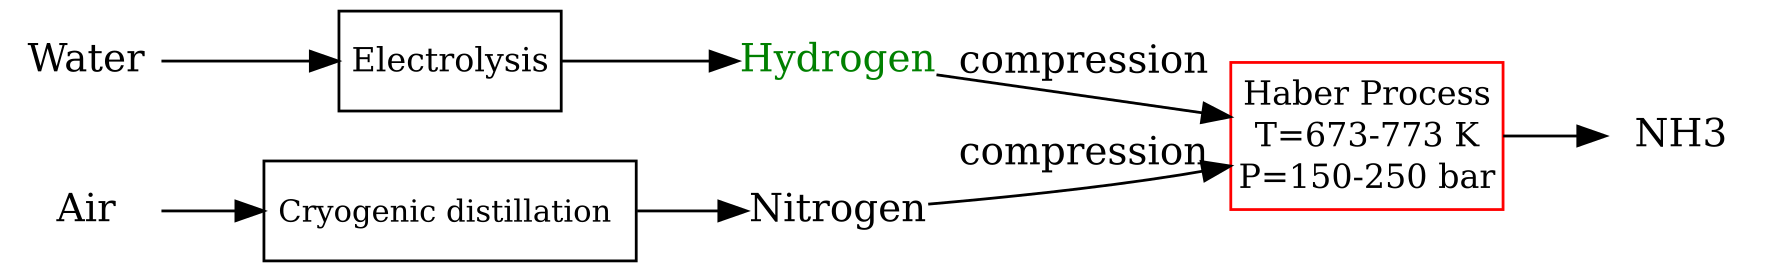
\includegraphics[width=12cm]{haber}

\caption{\label{fig:Haber-process}Haber process for the production of ammonia\cite{eftekhariQuantifyingRoleLiquid2020}}
\end{figure}

\sffamily \subsection{Methanol}
\normalsize
Methanol can be synthesized from the catalytic reaction of hydrogen
and carbon dioxide with the following reaction:
\begin{equation}
CO_{2}+3H_{2}\rightarrow CH_{3}OH+H_{2}O\label{eq:methanol}
\end{equation}
 The reactor operates at 100 bar and 264$^{o}$C \cite{luybenDesignControlMethanol2010}.
The reaction is exothermic and therefore the system is cooled down
by circulating water that produces steam. The material streams need
to be compressed to 50 to 100 bar in the reactor. Compared to methane
production in which two molecules of water is produced per molecule
of methane, only one molecule of water is produced during the reduction
of CO$_{2}$ to methanol. Therefore, even though the chemical exergy
of methanol is lower than that of methane, the synthesis of methanol
is slightly more efficient than the synthesis of methane. Similar
to the methane and ammonia production, the efficiency of methanol
synthesis is calculated by
\[
\eta_{methanol}=ex_{CH_{3}OH}^{ch}\left(\frac{3ex_{H_{2}}^{ch}}{\eta_{electrolysis}}+\frac{ex_{CO_{2}}^{ch}}{\eta_{capture}}+\frac{ex_{compression}}{\eta_{comp}\eta_{driver}\eta_{transmission}}\right)^{-1},
\]
which is estimated to be 40\%.

The subsurface storage of methanol, however, is not advisable since
methanol can be degraded by the subsurface microorganisms \cite{sousaDeepsubsurfaceSulfateReducer2018}.
Therefore, we did not include methanol in our subsurface model, although
only the input component name need to be changed in the attached Matlab
script to estimate the energy efficiency of the subsurface storage
of methanol (excluding the microbial degradation reactions). 

\begin{figure}[H]
\centering
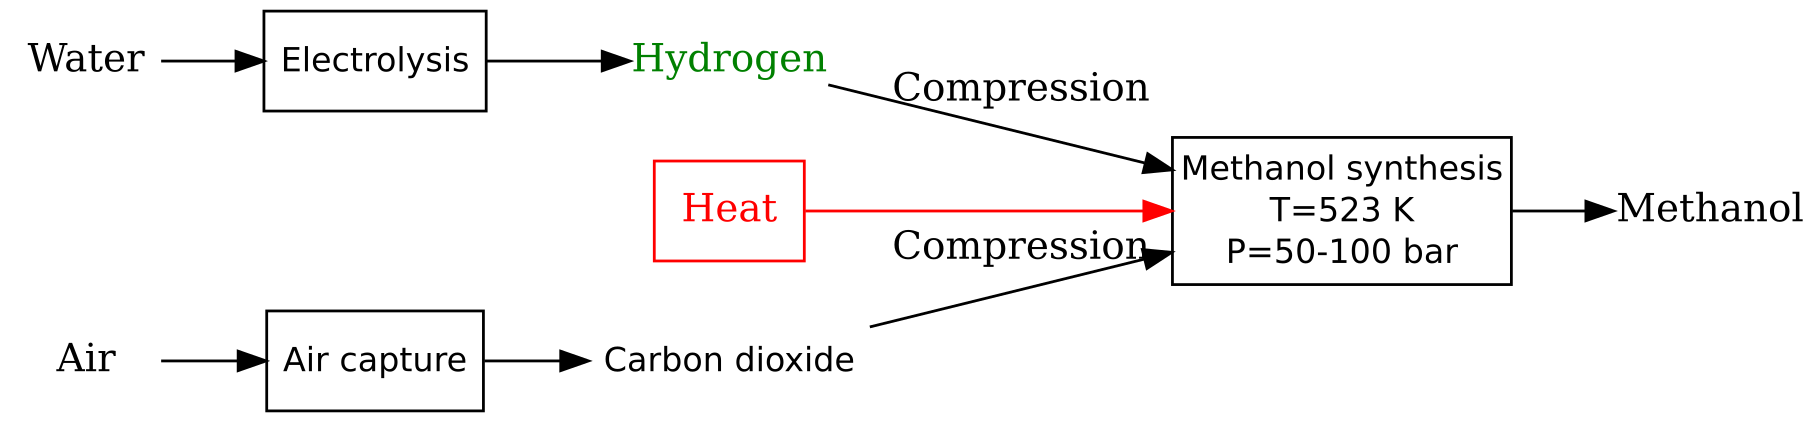
\includegraphics[width=12cm]{methanol}

\caption{A schematic of the methanol synthesis process \cite{eftekhariQuantifyingRoleLiquid2020}}
\end{figure}


\sffamily \section{Subsurface energy storage}
\normalsize
Although there are several reservoirs that can be used for the storage
of energy, we can divide them into two main groups of sandstone reservoir
(e.g. Harald West) and chalk reservoirs (e.g. Halfdan). Harald West
is a sandstone gas reservoir at a depth of approximately 3500 m and
a temperature of 135$^{o}$C. The porosity of the reservoir is 0.17
with a permeability of 1 to 50 mD in different layers. The thickness
of the two high permeable layers (9 and 54 mD) is approximately 100
m. The Halfdan chalk reservoir is 2000 m deep with an average porosity
of 0.31 and an average permeability of 3 mD. The wells in Harald West
are vertical and the chalk fields are typically producing through
long horizontal wells. In the case of a the vertical wells, we assume
a thickness of 100 m for the reservoir, which means that a radius
of 100 to 1000 m around the well will be utilized as the fuel storage
space. For the longer horizontal wells, a smaller area around the
well is required for the energy storage. We assume a well diameter
of 5'' for all the energy storage and production wells. 

\sffamily \subsection{Problem formulation}
\normalsize
We assume a gas reservoir represented
as a cylindrical domain. The top and bottom of the reservoir are closed,
i.e. no flow, and the outskirt of the domain can either be closed
or at hydrostatic pressure. The top side of the reservoir is located
at depth $L$ {[}m{]}, the thickness of the reservoir is $H_{res}$
{[}m{]} and the radius of the well and the reservoir are $0.5D_{well}$
{[}m{]} and $R_{res}$ {[}m{]} respectively. The injection rate is
calculated based on the surplus electricity and the efficiency factor
of the synthetic fuel production. The total injection
velocity is calculated by
\[
u_{inj}=\frac{E_{surpluss}\eta_{j}MW_{j}}{\pi D_{well}H_{res}ex_{j}^{ch}\rho_{j}},
\]
where $\rho_{j}$ {[}kg/m$^{3}${]} is the density of the synthetic
fuel $j$ and is calculated at the bottom hole pressure and injection
temperature (that is assumed to be close to the reservoir temperature).
The bottom hole pressure is unknown and is calculated by trial and
error between the reservoir model and the injection boundary condition
that is obtained from the above equation. The compression work
for the injection of the gaseous fluid is calculated for the injection
pressure of $p_{inj}=p_{bh}+\Delta p_{pipe}$, where $p_{bh}$ {[}Pa{]}
is the bottom hole pressure and $\Delta p_{pipe}$ {[}Pa{]} is the
pressure drop in the pipe that is calculated by the ``pipe'' unit
in the software Aspen Plus.

We assume that for 2 months from 1st of October to 1st of December
we only store the fluids in the subsurface (when surplus electricity
is available) and after that storage period, depending on the electricity
supply and demand we will have storage or production phases. The produced
fluid from the reservoir is used for the supply of the electricity
shortage; therefore, the withdrawal rate is determined by the electricity
shortage. If the withdrawal rate is too high, the reservoir might
not have enough driving force to produce the requested flow. In these
situations, the bottom hole pressure becomes negative and the program
produces an error. A better approach is to estimate the maximum productivity
of the reservoir using an analytical solution \cite{hagoortFundamentalsGasReservoir1988,al-hussainyApplicationRealGas1966,al-hussainyFlowRealGases1966}.
This approach is not currently implemented. 


\sffamily \subsection{Subsurface storage model}
\normalsize
For the storage of the synthetic fuels in the gas
reservoirs, we use a single-phase multi-component flow formulation.
The storage of gas in the water flooded reservoirs is not a good idea
since most of the gas will be trapped by capillary forces, and therefore
will be permanently stored. It is possible to dry out the reservoir
and prepare it for the gas injection by, e.g. injection of superheated
steam or hot gases. However, it will require large amounts of energy
and can potentially create thermally-induced fractures in the reservoir.
We will therefore consider only the gas reservoirs for the storage
of gaseous phase energy careers. For the liquid phase, we will use
both gas and oil reservoirs. In both cases, we will include the compressibility
of the fluids in the model as it is a major contributing driving force
in the extraction of the fluids from the reservoir.

The single phase compressible flow in porous media reads

\begin{equation}
\frac{\partial}{\partial t}\left(\varphi\rho\right)+\nabla.\left(\rho\mathbf{u}\right)=0,\label{eq:continuity}
\end{equation}
where the Darcy velocity (assuming single phase flow and negligible
gravity effect) is described by
\begin{equation}
\mathbf{u}=-\frac{k}{\mu}\nabla p,\label{eq:darcy}
\end{equation}
The flow of the synthetic fuel in the subsurface is described by the
advection-diffusion equation:
\begin{equation}
\frac{\partial}{\partial t}\left(\varphi c\right)+\nabla\left(\mathbf{u}c-\varphi\mathcal{D}\nabla c\right)=0.\label{eq:adv-diff-single}
\end{equation}
In the above equations, $\varphi$ {[}-{]} denotes porosity, $k$
{[}m$^{2}${]} denotes permeability, $\rho$ {[}kg/m$^{3}${]} denotes
the fluid density, $p$ {[}Pa{]} denotes the reservoir pressure, $\mu$
{[}Pa.s{]} denotes the fluid viscosity, $\mathcal{D}$ {[}m$^{2}$/s{]}
denotes the diffusivity of the synthetic fuel, and $c$ {[}mol/m$^{3}${]}
is the concentration of the synthetic fuel. Both viscosity and density
are functions of the fuel concentration. As discussed before, the
injection rate in the well is a function of the supplied electricity
that is obtained by the real surplus electricity data of 2020 adjusted
for 2050. The above equations are solved numerically with the finite
volume method. We performed the discretizition in the free Matlab
software package FVTool \cite{eftekhariFVToolFiniteVolume2015b} in
a two-dimensional axisymmetric (i.e. cylindrical) coordinate. We used
different permeability fields, including higher permeability near
the wellbore region. A version with the possibility of adding fracture
is also implemented.


\sffamily \section{Results and discussion}
\normalsize
In this section, we discuss the results of the ammonia storage in the Harald West field. A radius of 20
m around the well is stimulated to obtain a permeability 100 times
higher than the average permeability of the reservoir. This stimulation
is necessary for the injection of the large flow rates that are required
for the storage of energy in MW to GW scales. The withdrawal from
the reservoir starts on 1st of December 2050 whenever there is an
electricity shortage. The production rate is adjusted such that the
bottom hole pressure is high enough, i.e. it can overcome the pressure
drop in the well. We assume
that 100 MW of the surplus electricity is provided to the ammonia
production and storage unit in Harald West.
As can be seen in Fig. \ref{fig:Bottom-hole-pressure-NH3}, the injection
pressure in the reservoir is only 150 bar higher than the hydrostatic
pressure and thus within a reasonable range. The pressure fluctuation
is between 200 to 350 bar, which can create geomechanical failure
in the reservoir and needs to be further investigated. Once again,
the production rate is controlled by the low permeability of the reservoir
as can be seen in Fig. \ref{fig:Pressure-profile-NH3}. To avoid a
negative bottom hole pressure in the simulations, we imposed a withdrawal
rate limit that is 20\% of the maximum injection rate during the storage
phase. With this limit, the efficiency of the electricity production
(assuming an efficiency of 60\% for the conversion of ammonia to electricity)
from the stored ammonia is only 2.3\%, which does not provide the 72\% efficiency
that is required for a feasible storage solution that can address
the intermittency of renewable electricity production in the North
Sea windfarms.

\begin{figure}[H]
\centering
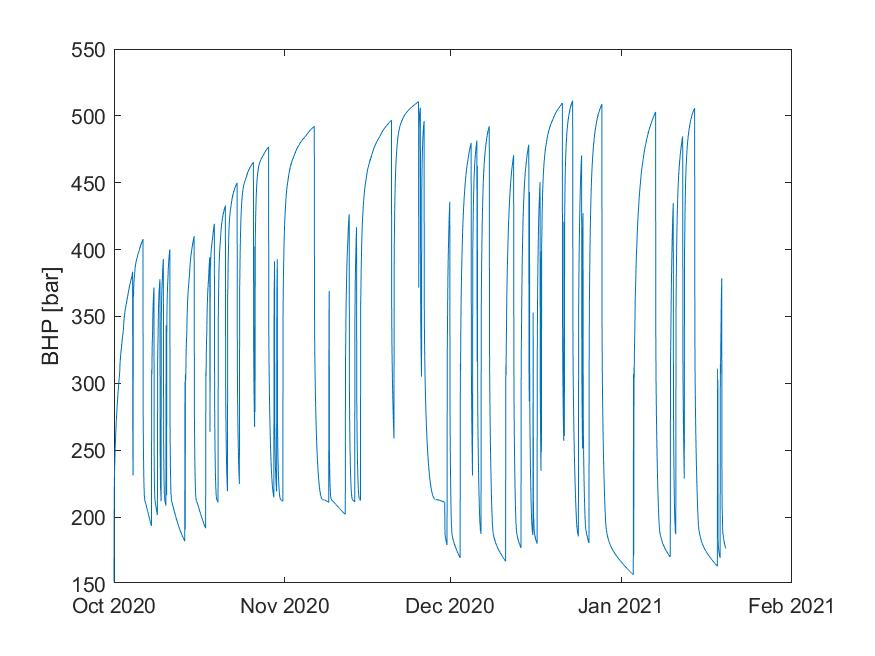
\includegraphics[width=8cm]{ammonia_p_hist}

\caption{\label{fig:Bottom-hole-pressure-NH3}Bottom hole pressure (BHP) of
the storage well in the Harald West ammonia storage facility}
\end{figure}

\begin{figure}[H]
\centering
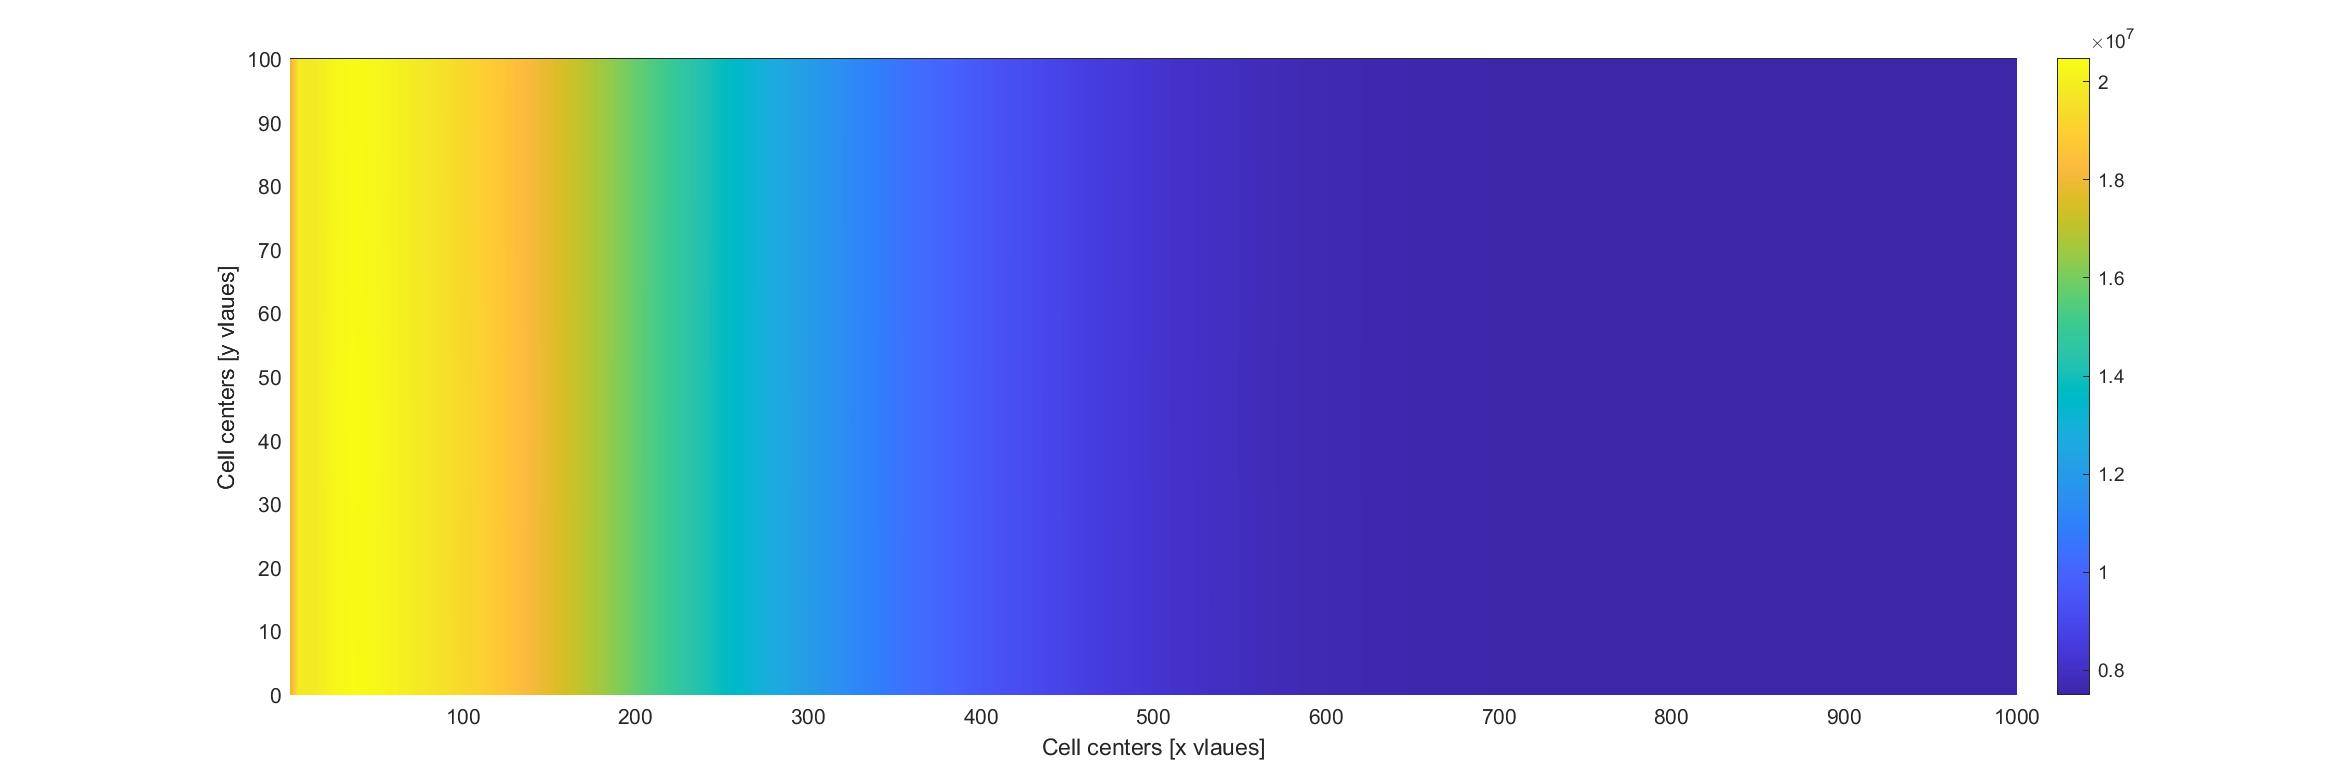
\includegraphics[width=14cm]{ammonia_pressure_harald}

\caption{\label{fig:Pressure-profile-NH3}Pressure profile in the reservoir
at the end of 4 months of ammonia injection and production}
\end{figure}

Finally, Fig. \ref{fig:concentration-profile-NH3} shows the normalized
concentration profile of ammonia in the reservoir after four months
of injection and production. Ammonia has diffused to a 300 m radius
around the well. Considering only the areas with a lower pressure
as non-reproducible zones and by integrating the concentration of
ammonia in those zones, an initial loss of 30\% can be expected for
the injected ammonia. We expect that the synthetic fuel loss in the
reservoir will not increase significantly and only occurs at the beginning
of the storage process in which the reservoir is pressurized for the
future re-production. 

\begin{figure}[H]
\centering
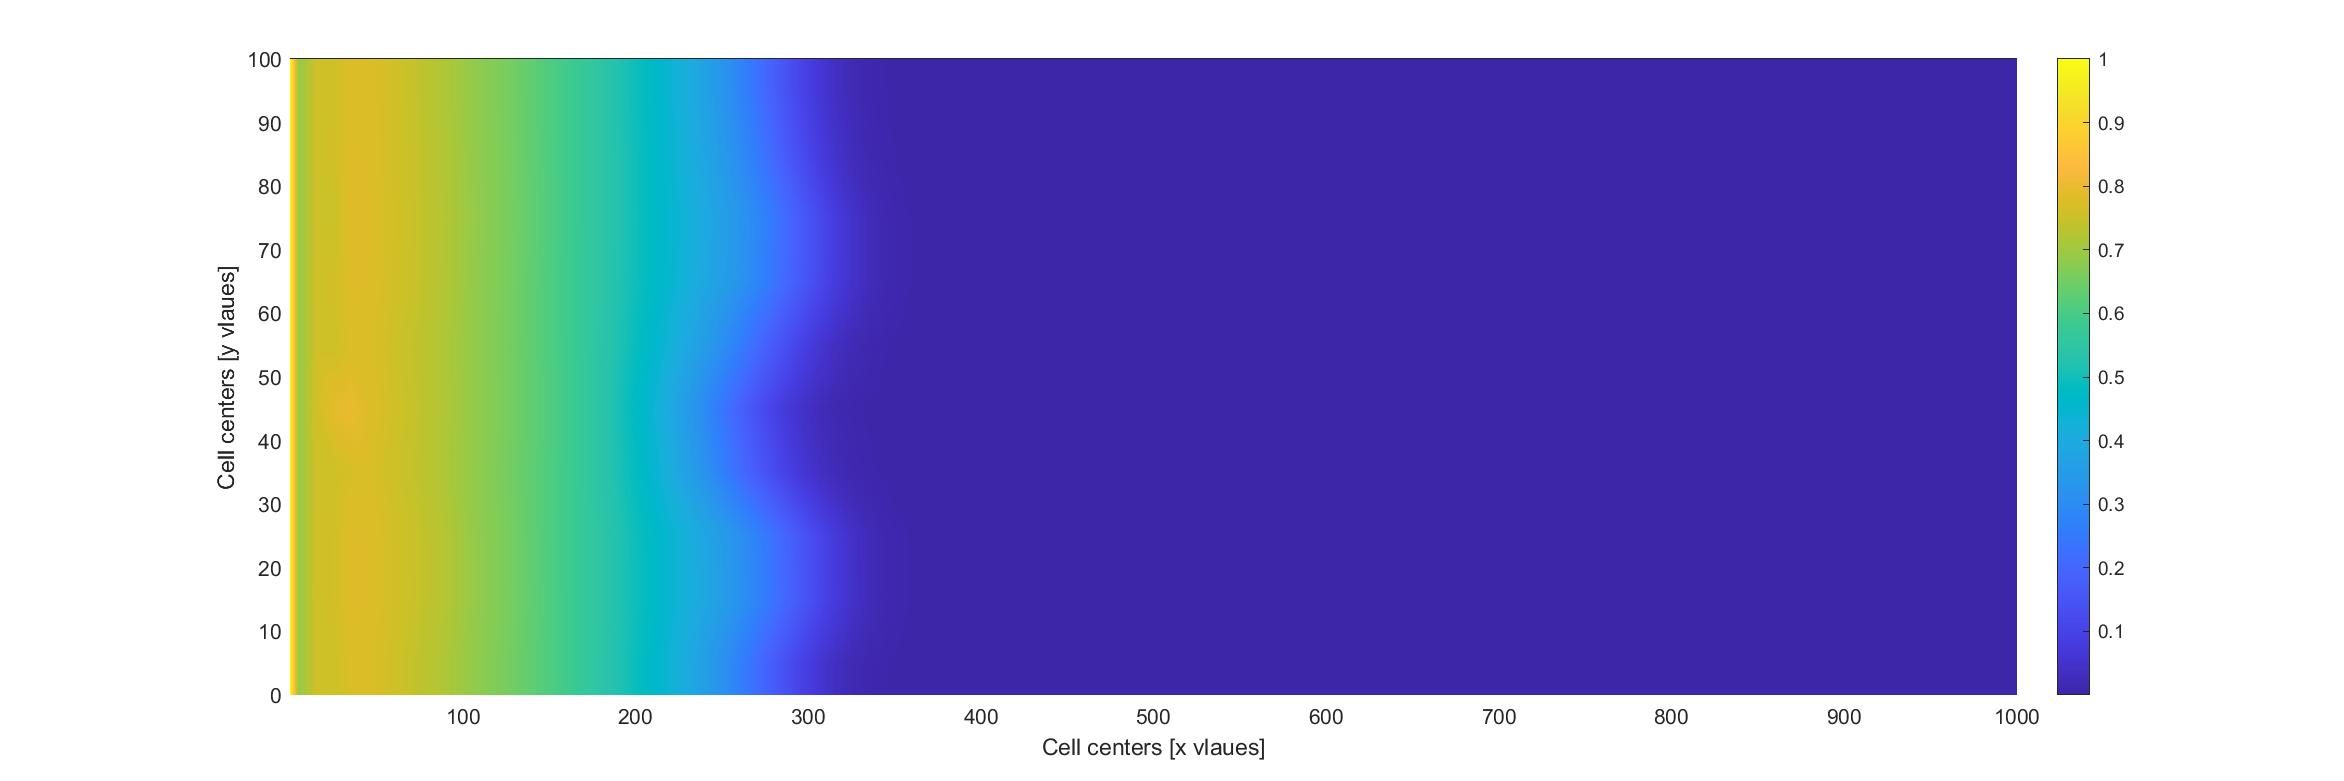
\includegraphics[width=14cm]{ammonia_tracer_harald}

\caption{\label{fig:concentration-profile-NH3}The concentration profile of
ammonia after 4 months of storage and withdrawal in the Harald West
reservoir}
\end{figure}

We repeated the simulations for the injection of synthetic fuels into a longer horizontal well; although the pressure
profile is different and the pressure fluctuation is significantly
reduced especially for the stimulated wells, the overall energy efficiency
remains unchanged. This implies that the subsurface storage of physical
and chemical energy must be performed in a confined zone, e.g. a salt
cavern, instead of a large reservoir in which the fluids can spread
due to the diffusive nature of flow in a porous medium.

\sffamily \section{Conclusions and suggestions}
\normalsize
In this paper, we studied the possibility of the subsurface storage
of the future surplus electricity that is produced in the North Sea
wind farms in the form of synthetic fuels to address the intermittency of the renewable
wind power. We showed that 
\begin{enumerate}
\item Any potential energy storage solution must have an energy loss of
less than 30\%. Currently, only hydropower storage and batteries offer
this efficiency, which are location dependent and only available in
smaller scales, respectively. None of the studied synthetic fuels,
with the possible exception of green hydrogen in certain conditions,
can be produced with the required efficiency.
\item For 2050, a capacity of greater than 1000 MW electricity storage is
required. The largest commercial hydrogen electrolysis units are in
the order of 20 MW and have a relatively large footprint that makes
them unsuitable for the offshore installations. Moreover, there is
currently no hydrogen gas turbine in the market and hydrogen can only
be utilized in hydrocarbon mixtures. 
\item Methanol and methane require a large carbon source, e.g. CO$_{2}$.
Air capture (the direct absorption of CO$_{2}$from the atmosphere)
is energy intensive and reduces the overall production efficiency
of the carbon-based liquid and gaseous fuels. They also have a large
footprint and do not fit on the offshore platforms. The only other
option is the capture and transportation of CO$_{2}$ from the point
sources by pipelines or ships to the platforms for the production
of methane and methanol. The production processes can fit easily on
a platform. 
\item Ammonia is the most promising fuel by a relatively high synthesis
efficiency and a low footprint (since it does not require a carbon
source). We introduced a new design that does not need cryogenic air
separation and is more suitable for the offshore ammonia production. 
\item Recuperation of the stored fuel with the desired flow rate is a limiting
factor in all the studied cases. It reduces the efficiency of energy
storage to the unfeasible values of 1-2\%. 
\item A confined subsurface space, e.g. a salt cavern, is a more realistic
alternative to the fuel storage in the North sea reservoirs.
\end{enumerate}

\sffamily \section*{Acknowledgment}
\normalsize
For their valuable discussion and support, AAE would like to thank
Charlotte Larsen and Charlotte Lassen and other colleagues in the
program management and technology maturation team at the Danish Hydrocarbon
Research and Technology Centre (DHRTC) at the Technical University
of Denmark. The research that led to this paper is funded by the
abandonment program of the DHRTC.

\sffamily
% \begin{thebibliography}{99}
\normalsize
\bibliographystyle{plain}
\bibliography{energy_storage}
% \end{thebibliography}

\end{document}
